\documentclass[10pt]{article}
\usepackage[a4paper,margin=1.6cm,top=1.3cm,bottom=1.3cm]{geometry}
\usepackage[T1]{fontenc}
\usepackage{lmodern}
\usepackage{microtype}
\usepackage{booktabs}
\usepackage{graphicx}
\usepackage{enumitem}
\usepackage{xcolor}
\usepackage[colorlinks=true,linkcolor=black,citecolor=black,urlcolor=blue]{hyperref}
\setlist{nosep,leftmargin=1.2em,topsep=1pt}
\setlength{\parindent}{0pt}
\setlength{\parskip}{3pt}
\pagestyle{empty}
\newcommand{\head}[1]{\par\smallskip{\large\bfseries #1}\par}
\newcommand{\sect}[1]{\par\smallskip{\bfseries\color{black!80} #1}\par}

\begin{document}
\head{Idea 11 PoC --- Waves of inexperienced investors and earnings news}
\textit{Proof of concept, October 2026. Code: \texttt{idea11\_new\_investors/run.py}.}

\sect{Question and design}
Inexperienced investors amplify bubbles (Greenwood and Nagel, 2009). In China, new investors' entries predict low
returns and explain daily momentum (Gao, Jiang, Xiong and Xiong, 2023). Do they also change how earnings news is
priced? If waves of novices amplify underreaction, the announcement-month response to surprises should fall and the
drift should rise in high-inflow months. The inflow measure is the monthly count of new A-share investors (CSDC,
via Eastmoney; public, no firm codes needed), in logs minus its trailing 12-month mean. It is available from April
2015, which gives 48 announcement months and 47{,}370 announcements up to October 2020. The longer proxy, 2005--2020,
is abnormal equal-weighted market turnover; its correlation with abnormal inflow is 0.54 over the overlap. The test
is a pooled regression of size-adjusted returns on SUE and SUE $\times$ proxy, with month fixed effects and SEs
clustered by month. The streak specification adds the gambler's-fallacy terms (SRW SUE, continuation dummy) and their
interactions with the proxy.

\begin{center}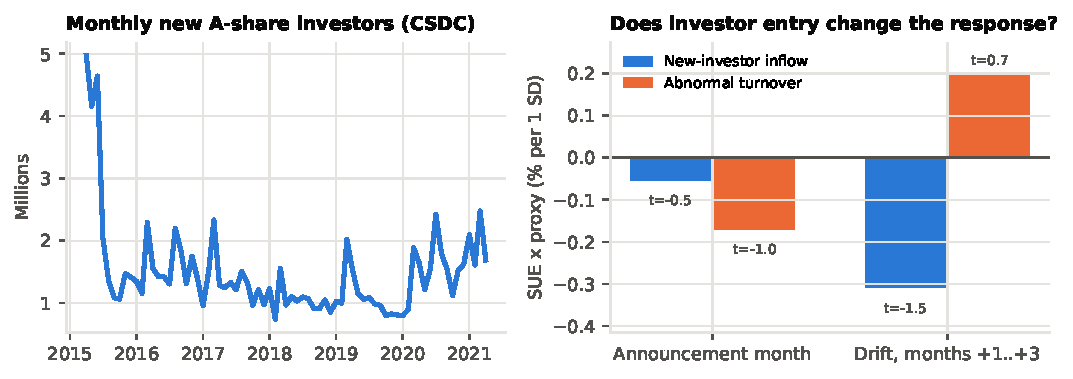
\includegraphics[width=0.97\textwidth]{results/fig_main.pdf}\end{center}

\begin{center}\small
\begin{tabular}{lcc}
\toprule
Interaction with SUE (\% per 1 SD of proxy) & Announcement month & Months $+1$ to $+3$\\
\midrule
New-investor inflow (2015--2020) & $-0.05$ ($-0.5$) & $-0.31$ ($-1.5$)\\
Abnormal turnover (2005--2020) & $-0.17$ ($-1.0$) & 0.20 (0.7)\\
Streak spec.: SUE$\times$cont.$\times$inflow & $-0.27$ ($-1.4$) & 0.05 (0.3)\\
\midrule
Drift slope, high- vs low-inflow months (29 months) & \multicolumn{2}{c}{0.08\% vs 1.08\% per 1 SD of SUE}\\
\bottomrule
\end{tabular}
\end{center}

\sect{Findings}
\begin{itemize}
\item \textbf{No evidence that novice waves amplify underreaction.} Neither the announcement-month response nor the
  drift moves significantly with new-investor inflow or abnormal turnover.
\item \textbf{If anything, drift is weaker when novices flood in.} In above-median inflow months the drift slope is
  close to zero (0.08\%), against 1.08\% in other months. In the streak specification the SRW drift slope falls with
  inflow ($-0.37$, $t=-2.0$). This fits attention-driven trading that speeds up incorporation, but the series is short.
\item \textbf{The streak effect does not vary with inflow either.} The gambler's-fallacy interaction is unrelated to
  novice entry, so the streak result does not appear to be driven by these waves.
\end{itemize}

\sect{Assessment and next steps}
Weak as a standalone paper with these data: only 48 announcement months with inflow data, and the turnover proxy is
not specific to novices. To revive it: (i) obtain the weekly CSDC series back to 2005 (Wind or CEIC) to cover the
2007 and 2015 waves; (ii) use cross-sectional exposure to novices (e.g.\ retail share, low price, lottery-like
stocks) and interact it with inflow; (iii) look at the speed of incorporation with daily returns, since the sign
here hints at faster pricing in hot markets. Lowest priority in Section~C.
\end{document}
